\chapter{Interpretability}

\begin{quote}
    In this chapter, we describe the experiments that were used to qualitatively analyse the features learned by the CLMR model, and get a deeper understanding of the model's learned representations.
\end{quote}

\section{Visualising Filters}
Figure \ref{fig:filter_visualisation} shows the magnitude spectrum of the learned filters of the sample-level convolutional layers (layers 1, 4 and 6) for CLMR and CPC, pre-trained on the MagnaTagATune and Billboard dataset.
In CLMR, the first layer is sensitive to a single, very small band of frequencies around 7500~Hz, while in higher layers, the filters spread themselves first linearly and then non-linearly across the full range.
CPC shows a similar pattern in the lowest layer, but shows a strong activation of two frequencies that span an octave.
Interestingly, CLMR shows a similar filter structure for the Billboard data set as fully supervised models that were trained on the MagnaTagATune dataset \cite{dieleman2014end,lee2018samplecnn}.
The Billboard dataset is significantly less diverse in genre, suggesting the self-supervised model focuses more on such frequency-band related differences than it does for the more diverse MagnaTagATune.


\begin{figure*}
    \centering
    \subcaptionbox{CLMR$^{(1)}_{\mathrm{MTAT}}$\label{fig:1a}}{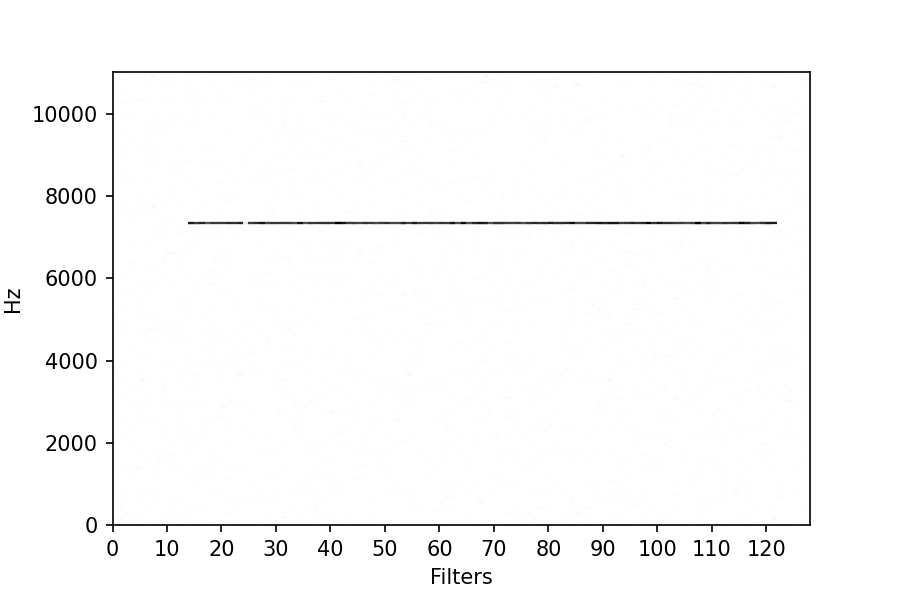
\includegraphics[width=.33\textwidth]{figs/magnatagatune/clmr_spectrum/epoch1490_layer0.png}}\hfill
    \subcaptionbox{CLMR$^{(4)}_{\mathrm{MTAT}}$\label{fig:1a}}{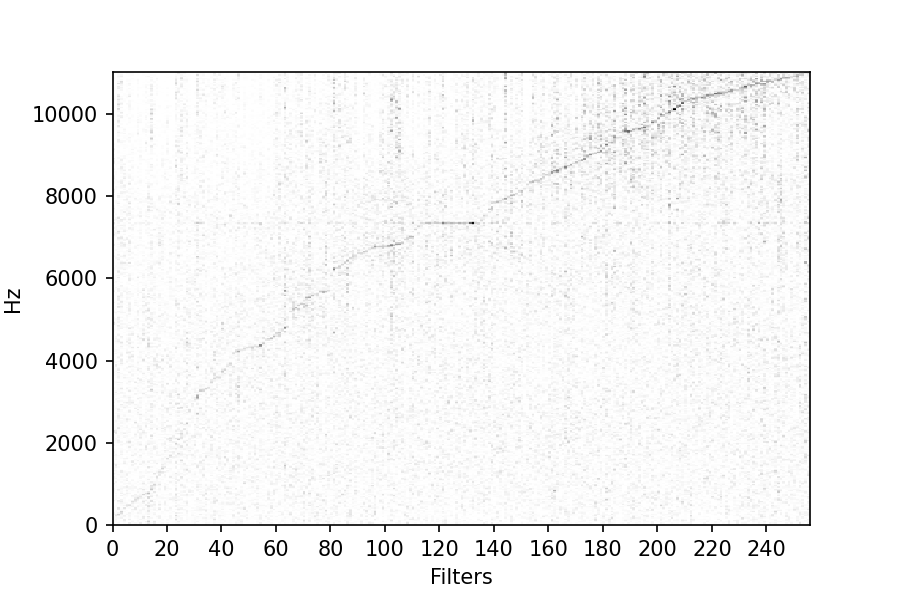
\includegraphics[width=.33\textwidth]{figs/magnatagatune/clmr_spectrum/epoch1490_layer3.png}}\hfill
    \subcaptionbox{CLMR$^{(6)}_{\mathrm{MTAT}}$\label{fig:1a}}{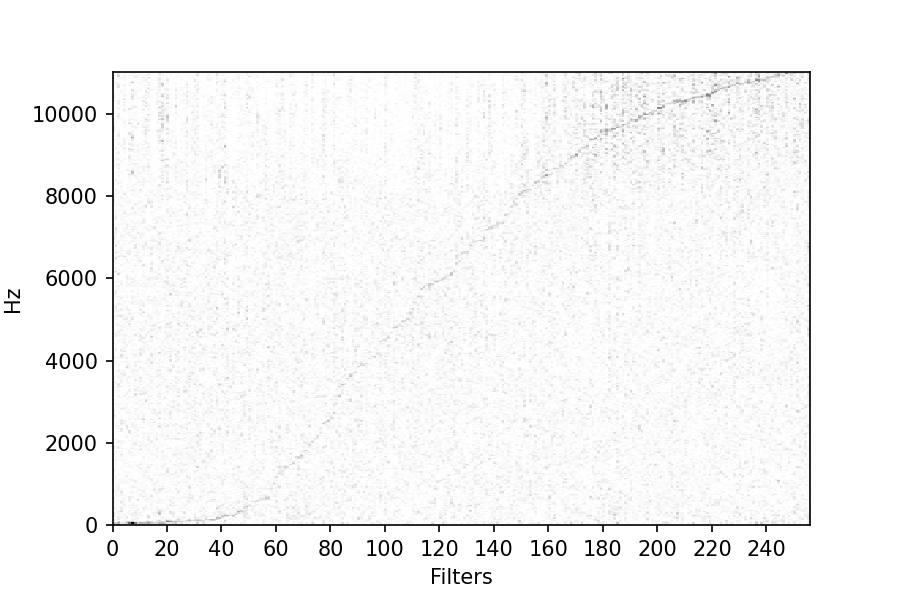
\includegraphics[width=.33\textwidth]{figs/magnatagatune/clmr_spectrum/epoch1490_layer5.png}}

    \subcaptionbox{CPC$^{(1)}_{\mathrm{MTAT}}$\label{fig:1a}}{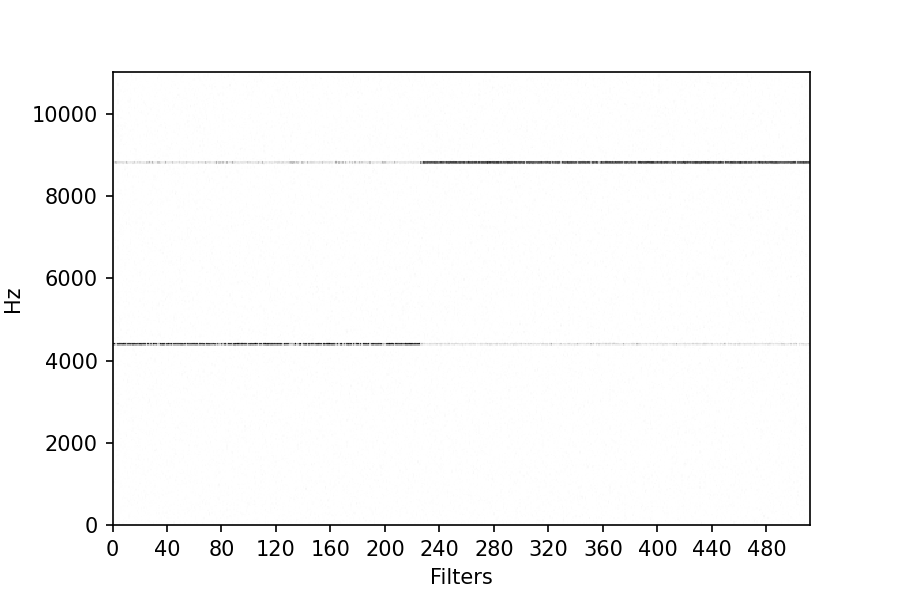
\includegraphics[width=.33\textwidth]{figs/magnatagatune/cpc_spectrum/epoch670_layer0.png}}\hfill
    \subcaptionbox{CPC$^{(4)}_{\mathrm{MTAT}}$\label{fig:1a}}{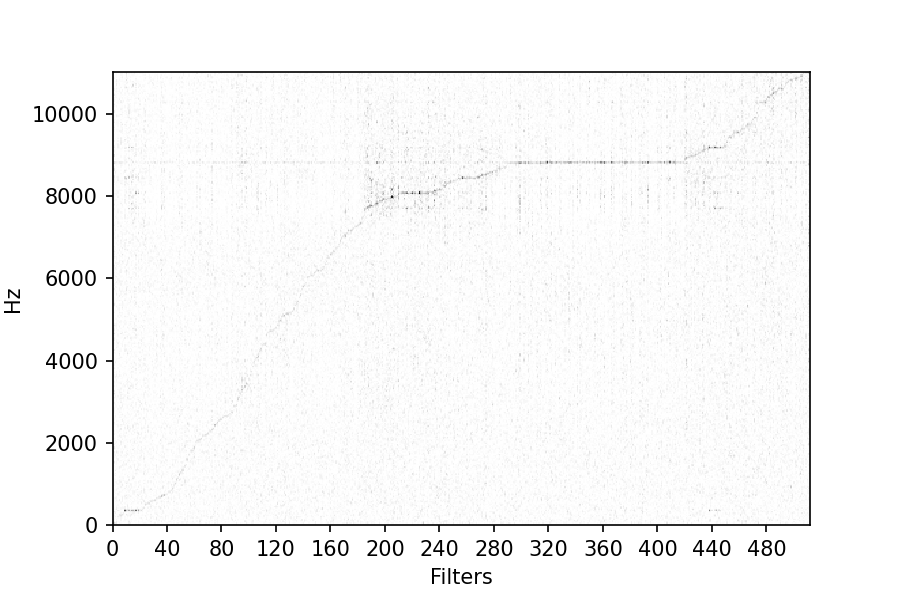
\includegraphics[width=.33\textwidth]{figs/magnatagatune/cpc_spectrum/epoch670_layer3.png}}\hfill
    \subcaptionbox{CPC$^{(6)}_{\mathrm{MTAT}}$\label{fig:1a}}{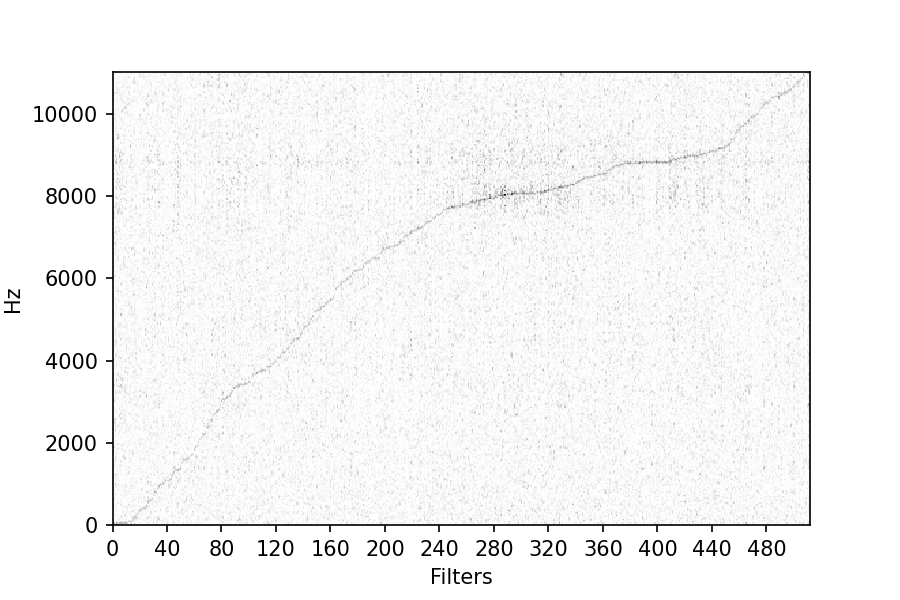
\includegraphics[width=.33\textwidth]{figs/magnatagatune/cpc_spectrum/epoch670_layer5.png}}

    \caption{Normalised magnitude spectrum of the filters of the self-supervised models in the sample-level convolution layers, sorted by the frequency of the peak magnitude. Gradient ascent is performed on a randomly initialised waveform of 729 samples (close to typical frame size) and its magnitude spectrum is calculated subsequently. Each vertical line in the graph represents the frequency spectrum of a different filter. The first three images are taken from a pre-trained, converged CLMR model, the last three from a CPC model}
    \label{fig:filter_visualisation}
\end{figure*}


\begin{figure*}
    \centering
    \subcaptionbox{CLMR$^{(1)}_{\mathrm{Billboard}}$\label{fig:1a}}{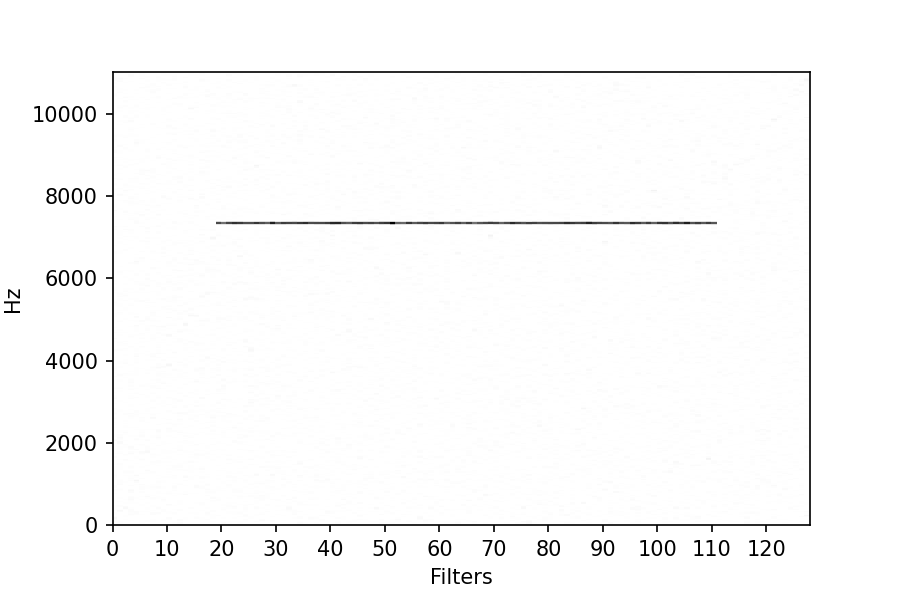
\includegraphics[width=.33\textwidth]{figs/billboard/clmr_spectrum/epoch1490_layer0.png}}\hfill
    \subcaptionbox{CLMR$^{(4)}_{\mathrm{Billboard}}$\label{fig:1a}}{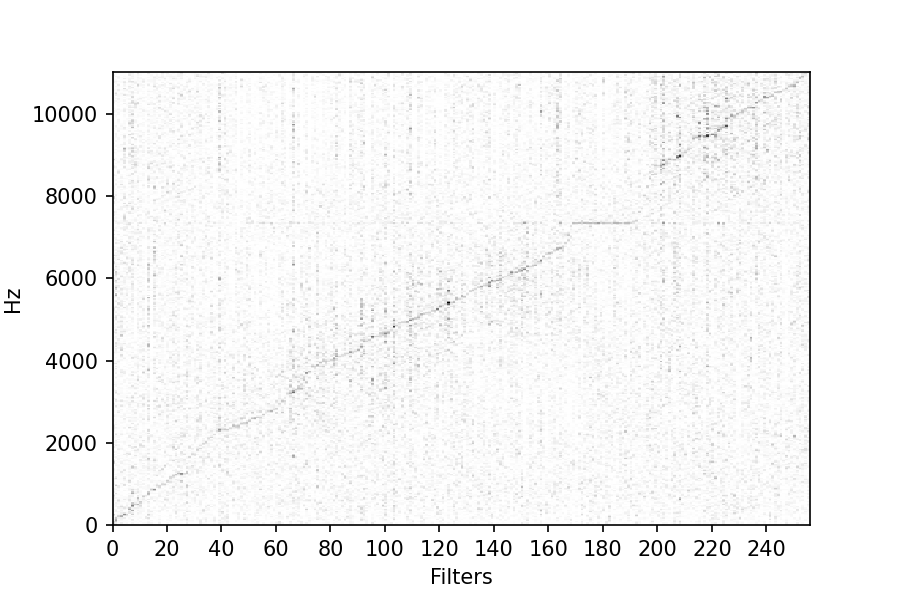
\includegraphics[width=.33\textwidth]{figs/billboard/clmr_spectrum/epoch1490_layer3.png}}\hfill
    \subcaptionbox{CLMR$^{(6)}_{\mathrm{Billboard}}$\label{fig:1a}}{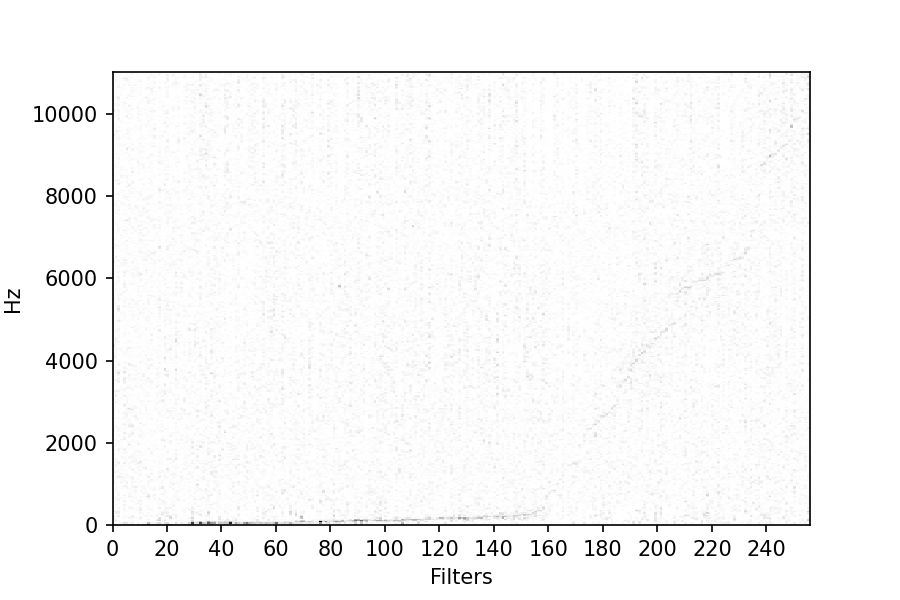
\includegraphics[width=.33\textwidth]{figs/billboard/clmr_spectrum/epoch1490_layer5.png}}

    \subcaptionbox{CPC$^{(1)}_{\mathrm{Billboard}}$\label{fig:1a}}{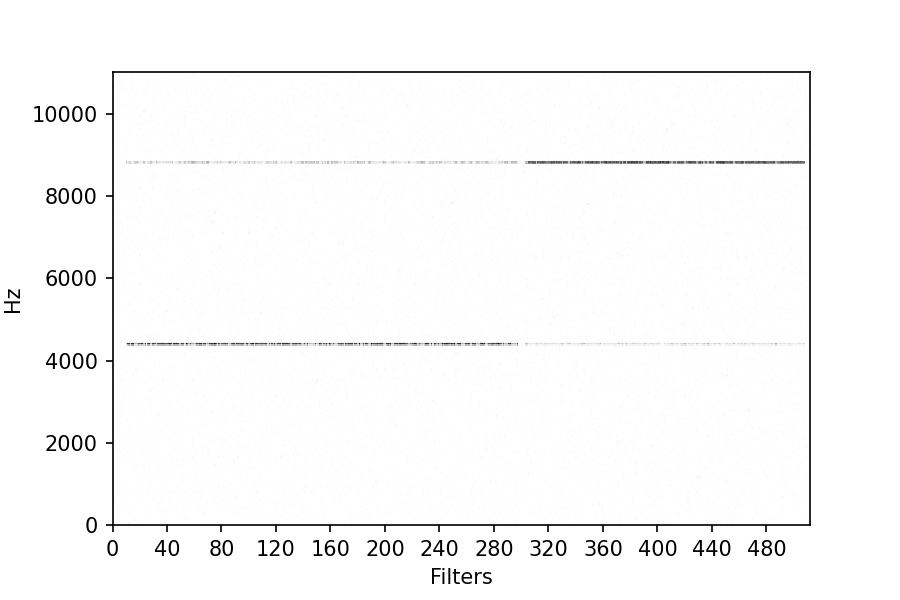
\includegraphics[width=.33\textwidth]{figs/billboard/cpc_spectrum/epoch1490_layer0.png}}\hfill
    \subcaptionbox{CPC$^{(4)}_{\mathrm{Billboard}}$\label{fig:1a}}{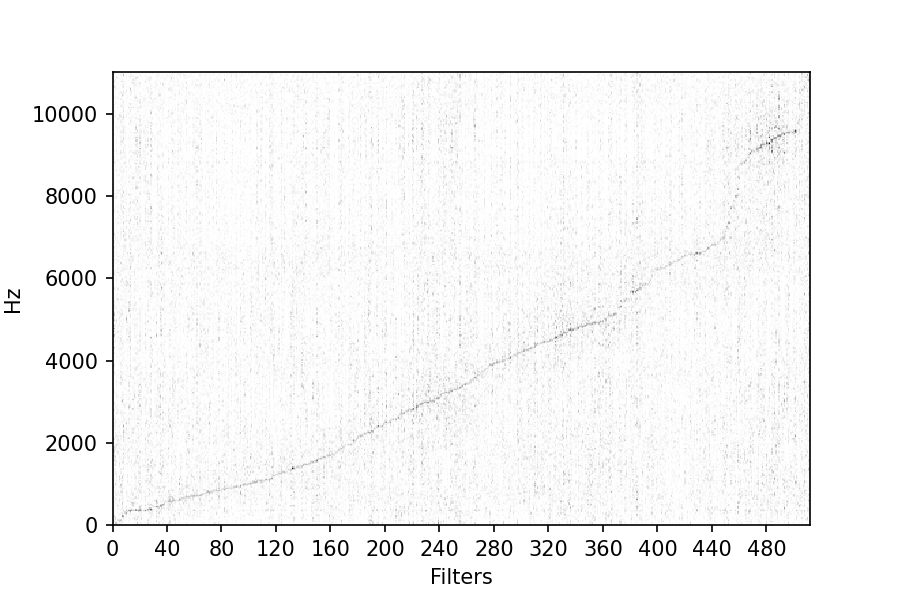
\includegraphics[width=.33\textwidth]{figs/billboard/cpc_spectrum/epoch1490_layer3.png}}\hfill
    \subcaptionbox{CPC$^{(6)}_{\mathrm{Billboard}}$\label{fig:1a}}{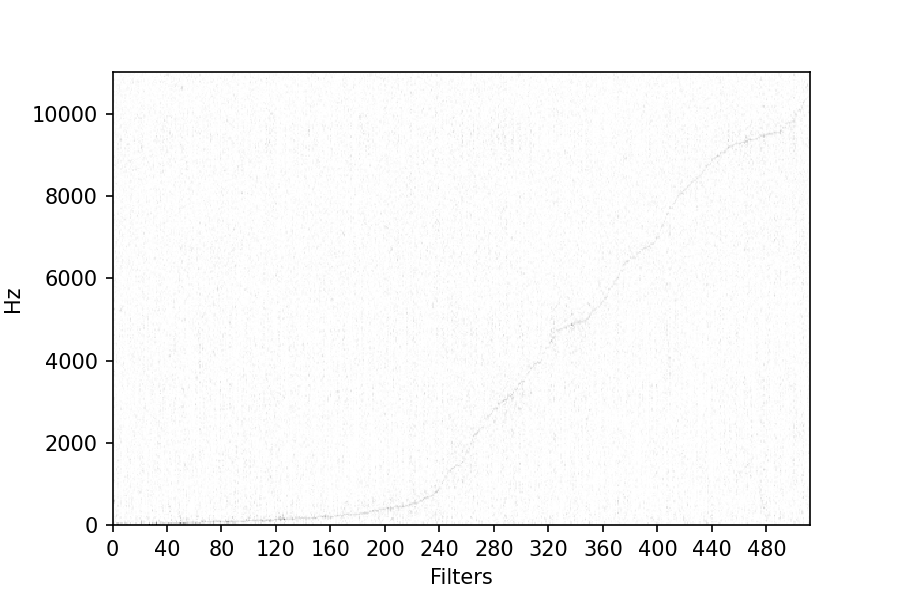
\includegraphics[width=.33\textwidth]{figs/billboard/cpc_spectrum/epoch1490_layer5.png}}
    \caption{}
    \label{fig:filter_visualisation_billboard}
\end{figure*}


% \section{Activations}
\begin{marginfigure}
    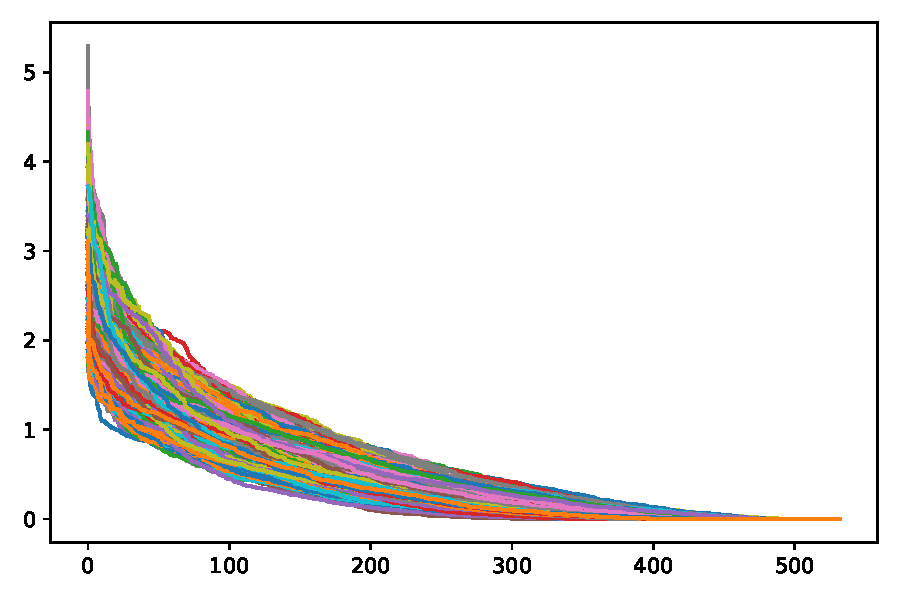
\includegraphics[width=\textwidth]{figs/activations.pdf}
    \caption{Mean activations of 512 features for every music segment, sorted by activation value.}
\end{marginfigure}

\section{Factor Analysis}
\begin{figure}[h]
    \centering
    \begin{subfigure}[b]{0.3\textwidth}
        \centering
        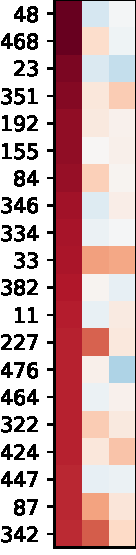
\includegraphics[width=\textwidth]{figs/varimax-magnatagatune-0.pdf}
        \caption{Component 1}
    \end{subfigure}
    \hfill
    \begin{subfigure}[b]{0.3\textwidth}
        \centering
        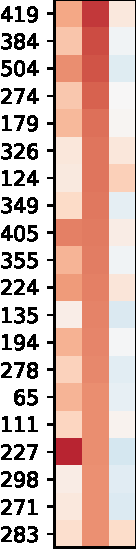
\includegraphics[width=\textwidth]{figs/varimax-magnatagatune-1.pdf}
        \caption{Component 2}
    \end{subfigure}
    \hfill
    \begin{subfigure}[b]{0.3\textwidth}
        \centering
        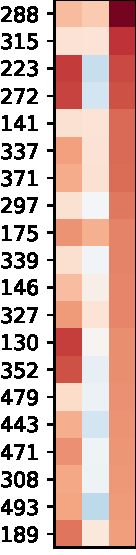
\includegraphics[width=\textwidth]{figs/varimax-magnatagatune-2.pdf}
        \caption{Component 3}
    \end{subfigure}
    \caption{Varimax rotation of 3 components on 512 factors (features) on a pre-trained CLMR model on the MagnaTagATune dataset. The figure shows the 20 strongest factors per component.}
\end{figure}


\section{Listening Experiment}
\begin{figure*}[h]
    \centering
    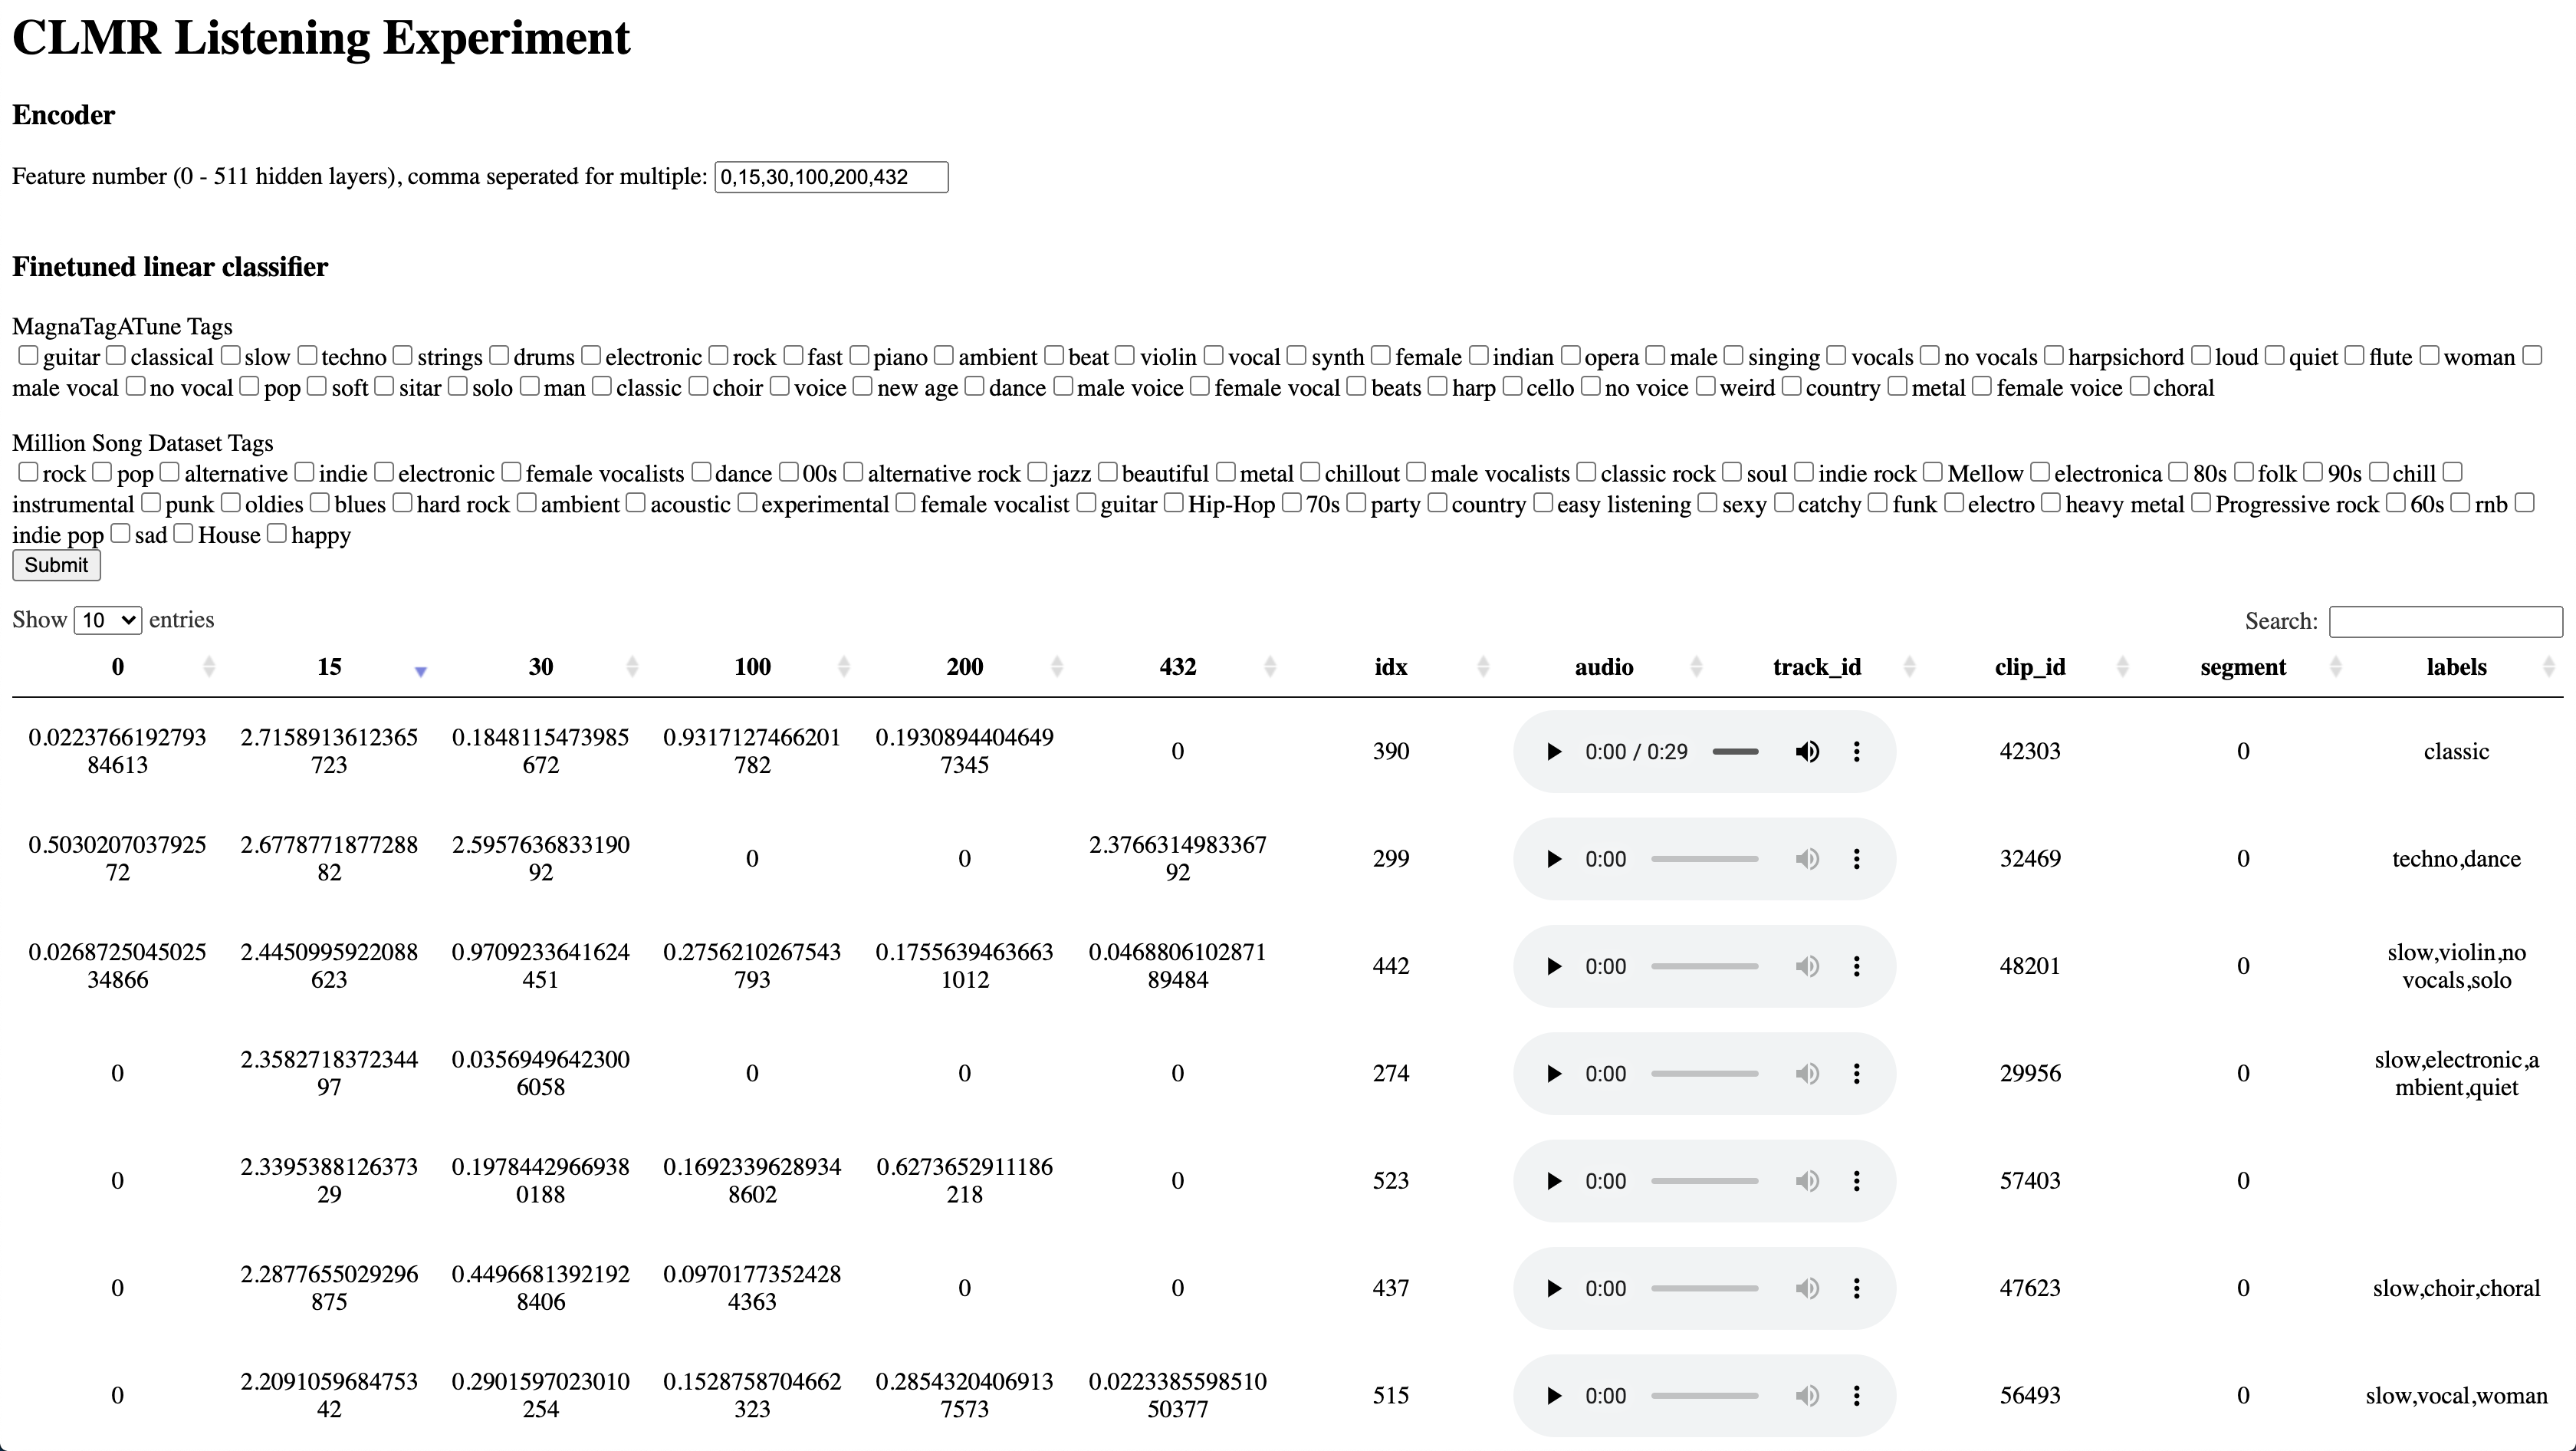
\includegraphics[width=\textwidth]{figs/listening_experiment.png}
    \caption{}
\end{figure*}